\documentclass[
  final,
  babelLanguage=portuguese,
  %desktopVersion,
  %showtrims,
  %overleaf,
]{anecdote}

%\graphicspath{{./assets/photos/300dpi/}}
\graphicspath{{./assets/photos/92dpi/}}

% Page size: 135mm x 120mm
% Body text: 11 / 13.6 pt

\usepackage{local}

%% Details of the book
%% ===================

\title{Dar Lugar à Intuição, à Revelação e à Visão Profunda}
\subtitle{}
\author{Ajahn Vajiro}
\publisher{Publicações Sumedhārāma}
\date{2026-04-03}
\editionInfo{\textit{Primeira edição}, 2026}
\ISBN{000-000-0000-00-0}

% === Metadata ===

\hypersetup{
  pdftitle={\thetitle},
  pdfauthor={\theauthor},
  pdfcopyright={Copyright (C) 2026, \thePublisher},
  pdfsubject={},
  pdfkeywords={},
  pdflicenseurl={https://creativecommons.org/licenses/by-nc-nd/4.0/},
  pdfcontacturl={},
  pdflang={pt},
}

%% === Load further packages ===

%% === Hyphenation exceptions and corrections ===

\hyphenation{London}

\begin{document}

\frontmatter

\ifdesktopversion
\desktopCover{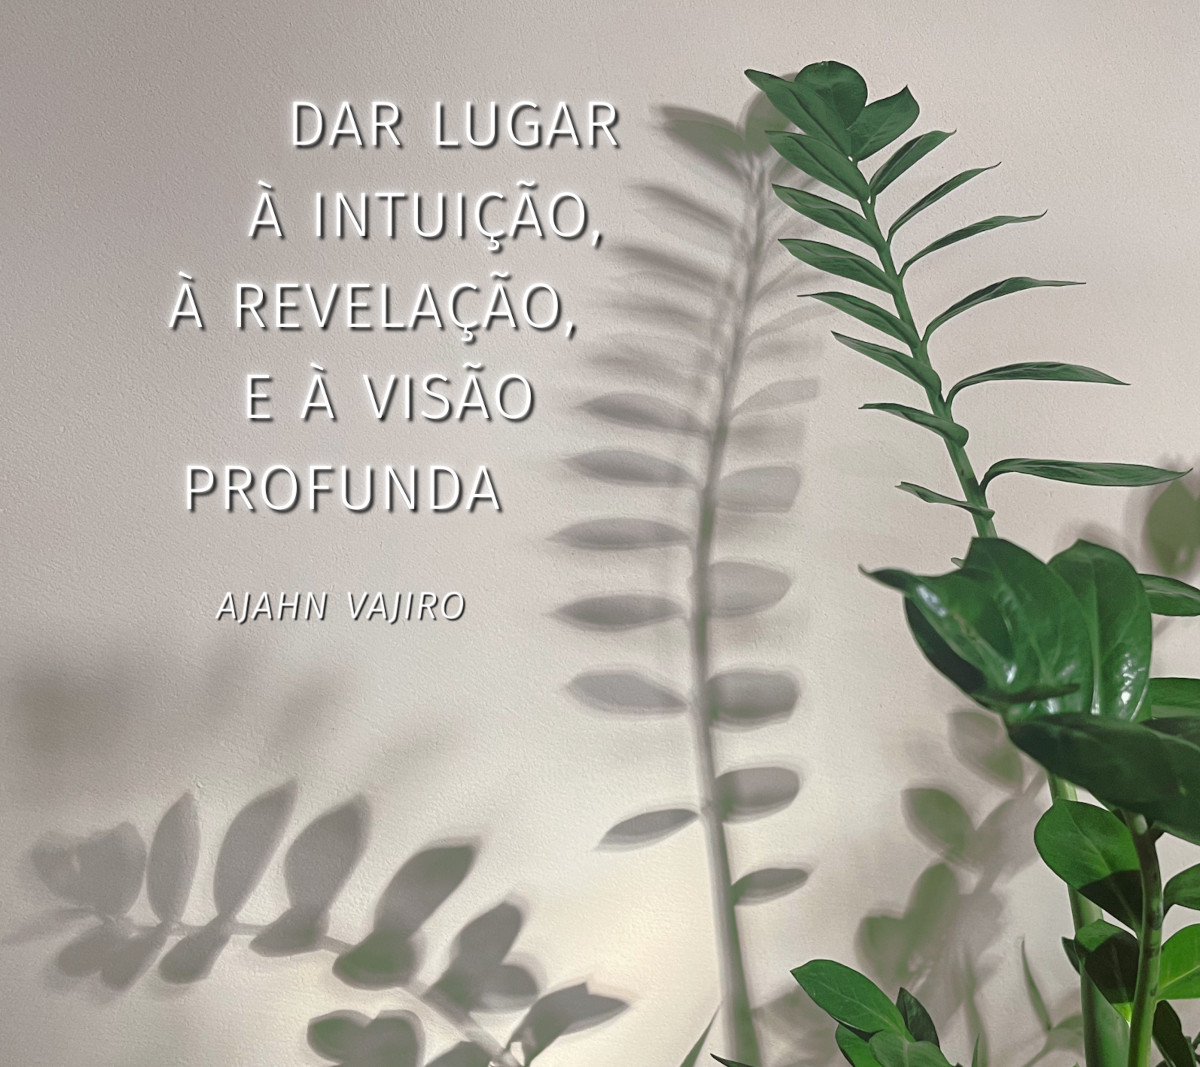
\includegraphics[height=\paperheight]{./desktop-cover-pt.jpg}}
\fi

\cleartorecto
\thispagestyle{empty}
\vspace*{5em}

{\centering

\settowidth{\titleLength}{%
  {\fontsize{13}{13}\chapterTitleFont\scshape\MakeLowercase{à Revelação e à Visão Profunda}}%
}

{\fontsize{13}{13}\chapterTitleFont\scshape\MakeLowercase{Dar Lugar à Intuição,\\[5pt] à Revelação e à Visão Profunda}}\\[0.3\baselineskip]
\setlength{\xheight}{\heightof{X}}
\raisebox{0.5\xheight}{\color[gray]{0.4}\rule{\titleLength}{0.25pt}}\\[0.3\baselineskip]

\vfill

{\fontsize{10}{10}\chapterTitleFont\selectfont \theauthor}

\vspace*{5em}

}



\cleartoverso
\thispagestyle{empty}

{\copyrightsize
\centering
\setlength{\parindent}{0pt}%
\setlength{\parskip}{0.8\baselineskip}%

\thetitle\\
por \theauthor

Published by \thePublisher

% No ISBN for the Portuguese edition
% ISBN \theISBN

Copyright \copyright\ \thePublisher\ 2023

This book is available for free download at\\
\href{https://sumedharama.pt}{www.sumedharama.pt}

\vfill

{\footnotesize

This work is licensed under a Creative Commons\\
Attribution-NonCommercial-NoDerivatives 4.0 International~License.

Produced with the \LaTeX\ typesetting system,\\ set in Gentium and Fira~Sans.

\theEditionInfo

}}


% \input{./manuscript/tex/dedication.tex}

% \cleartorecto
% \tableofcontents*

% \input{./manuscript/tex/foreword.tex}

% Page 1 is the first page of the first chapter.
\mainmatter

\chapter{Dar Lugar à Intuição,\\[5pt] à Revelação e à Visão Profunda}

{\centering
\begin{minipage}{0.8\linewidth}%
\centering\itshape
Este pequeno livro resulta de uma adaptação de uma sessão de Zoom oferecida por Ajahn~Vajiro
à Theosophical Society nos EUA, a 8~de~agosto de~2022.
\end{minipage}
\par}

\bigskip

\emph{Ajahn Vajiro:} Sejam muito bem"-vindos.

À medida que nos vamos juntando e serenando, vejo pessoas a chegar em alvoroço e
depois a tomarem a sua postura de ``agora vou estar consciente''. Mas lembrem"-se
e procurem recordar -- tal como eu o faço muitas vezes -- que a vida deseja o
bem para si própria, deseja o seu melhor.

Pode não estar certa do que é o melhor, ou pode não ter a capacidade para
encontrar o melhor, mas, inerentemente, a vida procura em permanência otimizar a
sua existência. Deseja o melhor para si. Porém, a verdade é que quando os seres
humanos desejam o melhor para si mesmos, podem estar muito confusos sobre o que
será, realmente, esse melhor.

Assim, quando nos encontramos numa ocasião como esta, em que se encoraja um
interesse e uma pesquisa interior mais profunda, é muito útil que mantenhamos em
mente a razão pela qual aqui estamos. E espero bem que não estejam aqui porque
se querem torturar a vós próprios! E espero que também não o estejam a fazer
porque querem discutir com os outros. Caso assim seja, lembrem"-se que estes são
modos confusos de nos desejarmos bem a nós mesmos. Portanto, proponho que façam
uma pausa e procurem conectar"-se com uma sensação interior profunda, a
experiência visceral de que ``este ser deseja bem a si mesmo''.

O estado mais elevado de felicidade, o bem"-estar mais completo para um
ser humano, consiste num estado independente de condições -- uma felicidade que
não se encontra dependente de quaisquer condições externas ou internas. Esse é o
estado mais elevado de felicidade.

Ajahn Buddhadāsa -- um monge tailandês muito conhecido e cujo nome significa o
``servo'' (ou ``escravo'') do Buda -- referia que quando os seres humanos agem
de forma correta, tornam"-se ``criadores de felicidade''. Uma bela aspiração que
vale a pena mantermos em mente.

Portanto\ldots{} o tema deste workshop foca"-se na ideia de podermos dar lugar à
intuição, à revelação e à visão profunda, e tentarei partilhar algumas reflexões
sobre a natureza do pensamento. E vou começar por estabelecer os paradigmas, as
perspetivas, de que modo podemos classificar um pressuposto como ``verdadeiro''
e sábio.

O Caminho Óctuplo começa com \emph{sammā-diṭṭhi} (visão correta) -- a premissa
de que, para nós, pessoas comuns, existe o ato da dádiva, da oferta e do
sacrifício; existem atos cujos resultados trazem felicidade, e atos cujos
resultados trazem mais dor; existe este mundo e existem outros mundos (outros
modos de experienciar a existência) que são diferentes, que não conhecemos
diretamente, existem seres que surgem espontaneamente; e nós temos ou tivemos
progenitores (e fomos cuidados por alguém); e existe quem -- no seio dos
contemplativos, ou outras pessoas que tenham praticado por si próprias -- seja
capaz de explicar estas matérias através da sua própria visão profunda.

\enlargethispage{\baselineskip}

Portanto, existem aqueles com quem é positivo e útil que nos associemos e
aqueles com quem não é. Podemos adotar estes pressupostos como estando em
sintonia com a verdade. Existem outros pressupostos que não estão em sintonia
com a verdade e quando nos associamos a estes e os colocamos em prática trazem
mais dor e mais confusão, tanto para nós próprios como para os outros.

Assim, o que vamos pôr em prática? E será que estamos cientes do que estamos a
praticar a nível inconsciente?

O segundo fator do Caminho é \emph{sammā-saṅkappa} -- por vezes traduzido como
``pensamento correto'' -- mas diria que uma tradução mais próxima do seu
verdadeiro significado seria ``resolução correta''.

\enlargethispage{\baselineskip}

Há uma opção que se toma. E esta ``resolução correta'' é ``\emph{sammā}'', que
significa que ``está de acordo com a Verdade''. Quando digo ``correta'' quero
dizer ``em sintonia com a Verdade''. Irei dar, a seu tempo, uma definição de
Verdade com que podemos trabalhar, sendo que ``Verdade'' consiste numa das
formas encontradas para traduzir Dhamma por um único vocábulo. Dhamma é algo
precioso ou seguro. O Dhamma consiste numa das partes da tríade: Buddha, Dhamma,
Sangha. \emph{Sammā-saṅkappa} consiste no pensamento ou na resolução que se
encontra de acordo com o Dhamma. Podemos optar e praticar a tomada de decisões e
a elaboração de pensamentos que estejam em sintonia com a Verdade.

A descrição deste processo é interessante, pois, como talvez já possam ter
reparado, muito do que se relaciona com o Budismo aparenta ser negativo, mas
isso prende"-se com o facto de que é mais fácil repararmos naquilo que parámos de
fazer, que repararmos naquilo que estamos a fazer. Portanto, a resolução correta
é aquela que começa por decidir renunciar, decidir não ceder; decidir não ser
cruel nem explorar os outros; e decidir não fazer mal. Assim, sempre que
repararmos que as nossas ações estão a ir nessa direção, é porque não estamos a
agir em sintonia com o Dhamma, não estamos em sintonia com a Verdade. É~muito
fácil verificar o espaço e a tranquilidade inerentes a uma vida de renunciante,
sem crueldade nem fazer~mal.

Uma forma de conseguirmos ganhar alguma perspetiva sobre o que é amplo e
silencioso é procurar experienciar o neutro. Isto porque muito facilmente não
prestamos atenção ao que é~neutro. E existe uma experiência neutra a que muito
facilmente não prestamos atenção e que é incrivelmente importante: este ritmo
peculiar com que vivemos 24 horas por dia -- a inspiração e a expiração. Este
movimento é uma experiência neutra e algo muito importante, porque se não
estivermos a respirar, estamos em apuros! Portanto, durante esta primeira parte
em que estamos juntos, proponho que dediquemos algum tempo a praticar estarmos
conscientes do que é neutro, dedicando uma atenção cuidada e carinhosa à nossa
inspiração e à nossa expiração.

\section{Meditação Guiada}

\enlargethispage{\baselineskip}

Agora, tomem a posição que quiserem -- de pé, a caminhar, sentados ou deitados.
Seja qual for, sugiro que escolham aquela postura que vos dê uma sensação de
desbloqueio. Ou seja, podemos começar por pensar que temos de nos agarrar a uma
postura que temos de manter, mas aquilo que prefiro sugerir é que se procure a
postura que nos faça sentir desbloqueados, soltos.

Mantenham"-se alerta e direitos, com os olhos abertos ou fechados, acolhendo cada
inspiração e soltando cada expiração\ldots{} aceitem o ritmo da respiração e
ofereçam"-lhe o dom da atenção sem qualquer expetativa, remorso ou medo\ldots{}

Atentem se a respiração é longa ou curta, se é uma inspiração ou uma
expiração\ldots{} e mantenham"-se apenas na consciência deste saber\ldots{}
ofereçam vida à vida\ldots{} sem qualquer tipo de remorso ou preocupação ou
esperança, ou medo\ldots{}

Permitam que esta atenção e esta experiência sejam totalmente desbloqueadoras.
Sintam como o corpo se aquieta à medida que toda esta experiência é recebida e
desbloqueada através do dom da atenção\ldots{} reparem como há uma felicidade
suave que se revela, que se reconhece e realiza\ldots{}

\enlargethispage{\baselineskip}

Permitam também que os padrões e ritmos do coração se possam revelar\ldots{} e
nessa revelação há uma calma que permitimos que se instale\ldots{} à medida que
o coração se revela naturalmente, permitam que este se eleve, permitam à
expiração que se solte e libertem"-na muito suavemente. Prendam a respiração por
um momento e de seguida tornem a inspirar, sorvendo a inspiração de novo à
medida que é recebida\ldots{}

Mantenham"-se neste estado de compostura, de circunspeção, sustendo a atenção. Ao
mantermos o coração recolhido desta forma, podemos reparar como a experiência é
toda ela inconstante, variável, naturalmente incerta e, portanto, algo que não
deveremos levar tão a sério -- tão pessoal -- deste modo permitimos, e damos
espaço para que possa ser tal como é, e que possa também terminar\ldots{} e,
assim, reparamos na forma como as coisas também terminam, neste espaço e neste
tempo\ldots{} como as coisas terminam\ldots{} a respiração é assim\ldots{} a
vida é assim\ldots{} aqui e agora\ldots{}

\enlargethispage{\baselineskip}

E esta é uma forma de darmos espaço e tempo, aqui e agora, à intuição, à
revelação e à visão profunda.

\bigskip

{\centering
\textit{(Final da meditação guiada)}
\par}

\bigskip

Os seres humanos têm a capacidade de direcionar o pensamento e de orientar
conscientemente as suas volições e intenções. A volição e a intenção, no que se
refere aos ensinamentos do Buda, baseiam"-se na visão correta: no facto de que
existem pensamentos e ações que são benéficos e que levam a resultados
benéficos, e que existem pensamentos e ações que são inadequados e que levam a
resultados inadequados. As volições e as intenções são causas. Existem causas e
condições; quando existem as causas e as condições para que algo se revele, tal
irá revelar"-se, e sempre que as causas e as condições não se encontrem para que
algo se revele, tal não se irá revelar. É tão simples como isso.

Bastou ao discípulo mais sábio do Buda escutar estas palavras para que este
chegasse ao entendimento inicial. Este entendimento ou realização consiste na
premissa inicial do Caminho Óctuplo, ou seja, a ``visão correta''. Esta visão
baseia"-se na ideia de que ao realizarmos atos positivos e generosos, existirão
bons resultados. Este tema é repetido ao longo de todos os fatores do Caminho
Óctuplo; todos os fatores do caminho são como uma prescrição para a cura de todo
o stress e tensão da condição humana. Os ensinamentos do Buda começam com aquilo
que todos nós conseguimos identificar: a condição humana da irritação, dos
stresses, das tensões; a discórdia e a doença, e a separação e o conflito. O
Caminho Óctuplo, ou Via Óctupla, oferece uma prática para mitigar ou remover as
causas para todos os acrescentos desnecessários que nos aumentam o stress e a
tensão. E os ensinamentos oferecem"-nos, ainda, orientação para que saibamos como
nos relacionarmos com a nossa condição humana de modo que esta se torne numa
existência nobre e em algo que realmente valha a pena.

Onde quero chegar é à visão correta, que nos oferece perspetivas úteis,
pressupostos e um paradigma. Gosto de dar um sentido mais vasto a ``visão'',
porque o termo \emph{diṭṭhi} inclui a forma como olhamos para as coisas, e o
modo como abordamos as coisas; é ativo. Peguemos, por exemplo, na perspetiva de
que vimos de algum lado: esta perspetiva recorda"-nos que houve alguém que cuidou
de nós no início da nossa vida. Portanto, de uma forma ou de outra, o comum dos
seres humanos recebeu algum tipo de cuidado. Fomos criados por alguém. Se um
ser humano não for criado por alguém, morre. Portanto, se estão vivos, é porque
alguém vos criou. E este é um bom início onde basear as nossas perspetivas.

Para além disso, existem coisas que não compreendemos -- estados, causas e
condições sobre os quais não temos a menor ideia. É bom que nos recordemos
disto, porque se pressupomos que sabemos tudo, e que compreendemos tudo, então
iremos cair na armadilha de achar que nunca cometemos erros. E só pessoas muito
imbecis acham que nunca cometem erros. Outro nível de imbecilidade é não saber
aprender com os nossos erros. Se formos um bocadinho inteligentes, aprendemos
com os nossos erros. Se formos ainda mais espertos, tentamos aprender com os
erros dos outros -- chama"-se a isso ``educarmo"-nos a nós próprios''. É útil,
portanto, partir do pressuposto que não sabemos tudo; conseguirmos reconhecer 
tal facto é uma faculdade em si: saber que não sabemos.

Os seres humanos têm a capacidade de saber que não sabem. E logo de seguida vem
a capacidade para se aperceberem que pode existir uma forma de aprender. E,
finalmente, existe a faculdade da fé, em acreditar que poderá existir alguém com
quem possamos aprender. Estas tomadas de consciência formam a base e consistem
no ponto de partida para a sabedoria. Com base nesta sabedoria, poderemos então
tomar resoluções e desenvolver pensamentos que poderão ser benéficos e
salutares, com os resultados subsequentes. Quando geramos pensamentos -- ou
seja, intenções deliberadas -- que não são benéficos, estes produzem resultados
tão pesados como as rodas de uma carroça carregada, puxada por um animal de
carga; quando geramos pensamentos benéficos, estes produzem resultados tão leves
como uma sombra.

Portanto, nós podemos decidir renunciar, podemos decidir não nos deixarmos levar,
podemos decidir não sermos cruéis ou explorar os outros; podemos decidir não
causar dano, e lembrem"-se que quando nos deixamos levar, estamos a causar dano a
nós próprios. Quando decidimos diretamente magoar, ser cruéis ou explorar os
outros estamos, imediata e diretamente, a nos dessensibilizar. Quando nos
deixamos levar pela satisfação dos sentidos, estamos a sobrecarregar os sentidos
ao ponto de os tornar dormentes, estamos a dessensibilizar"-nos, tal como
quando decidimos ser cruéis, magoar ou explorar outros seres. Toda a nossa vida
se baseia em sermos sensíveis e em reagirmos à sensibilidade. A vida é preciosa.
O que vos propus que fizessem no primeiro pequeno exercício de meditação foi que
respirassem sentindo tudo isto. Saber se estamos a inspirar ou a expirar é um
bom indicador, uma boa base. Portanto sempre que se sintam desconjuntados, ou
confusos, podem sempre verificar se estão a expirar ou a inspirar. E enquanto
expiram e inspiram, podem notar se essa respiração é longa ou curta. Esta ação é
sempre possível, o que quer que estejam a fazer. E através da ação contínua
dessa atenção, desse saber, a vossa vida irá transformar"-se. Eu prometo. Porque
o que irá surgir, entretanto, será um interesse crescente em manter a atenção
focada sobre todo o processo da respiração, sobre todo o corpo que respira --
toda a experiência em redor deste aspeto tão importante da~vida.

\enlargethispage{\baselineskip}

Como é que o corpo respira? Enquanto isto que aqui está se mantiver vivo, vai
estar a fazer isto: inspirar e expirar -- é assim, o seu ritmo básico. Não o
controlamos -- ambas têm de acontecer. E a forma como nos relacionamos com esta
ação é~muito reveladora. Revela toda a espécie de estados emocionais e tensões.
E podemos até jogar com a respiração. Experimentem expirar trazendo o abdómen
para dentro enquanto expiram; parem no final da expiração. De seguida, inspirem
o ar à medida que estendem o abdómen. Tentem fazer isto por alguns minutos e
vejam o que acontece. Depois vão experimentando uma respiração longa e uma
respiração curta. Vejam que efeito isso tem, e qual o interesse que existe
nisso, e vejam como os hábitos da mente se revelam.

Quando nos habituamos a reparar em algo neutro como a respiração, permitimo"-nos
reparar naquilo que é importante e em que normalmente não reparamos, aquilo que
não acolhemos e a que não oferecemos atenção. O importante é notar quando os
pensamentos cessam. Reparar nisso é importante, porque o nosso pressuposto é que
viver é pensar. Mas há algo que não é pensamento. E existe espaço em redor do
pensamento. Cada pensamento tem um início e um fim. Portanto, começamos a
reparar naquilo que usualmente não reparamos. O silêncio. O espaço. O que não
está a pensar?

Talvez seja boa ideia, agora, que eu ofereça uma definição de ``Verdade''. No
Budismo, chamamos"-lhe ``Dhamma''. Este termo ``Dhamma'' é traduzido de diversas
formas. O meu mestre traduz muitas vezes como ``as coisas tal como são''. Nas
escrituras é diversas vezes descrito como algo que ``é revelado pela
sabedoria'', ``revelado pelo mestre supremo, o Buda''. A Verdade existe por si
só, quer tenha sido apreendida por nós ou não. A Verdade é algo que é imanente,
que está aparente aqui e agora. A Verdade é este aqui e agora. É algo que existe
sempre no momento presente, neste tempo e neste espaço. E é também eterno, é
exterior ao tempo. O Dhamma não está circunscrito ao tempo nem ao espaço.

O pensamento está totalmente conectado ao tempo. Está constantemente a querer
interpretar e simplificar, e cai rapidamente na proliferação. E está preso ao
tempo. Pelo contrário, o Dhamma, enquanto refúgio precioso, não está preso nem
no pensamento, nem pelo pensamento; está fora do tempo e do espaço.

\enlargethispage{\baselineskip}

A Verdade encoraja e convida à investigação. Poderá ainda não se ter revelado,
mas, ao mesmo tempo, ela não está oculta. E é bela. Ao reconhecermos a Verdade,
ao nos apercebermos da Verdade, há uma sensação de descoberta de uma beleza que
esteve sempre ali, escondida à vista de todos.

E aí, mesmo tudo aquilo que possa parecer horrível ou nojento, é acompanhado de
um conhecimento, de uma observação: ``é assim que isto é'' -- e somos encorajados
a investigar, e a ganharmos um poder de observação e uma capacidade que permite
apercebermo"-nos: ``Foi assim que isto se desenrolou\ldots{} foi isto que
aconteceu, é assim que isto é''.

A libertação ou descontração que surge com esta tomada de consciência é um
aspeto da Verdade. Leva a mente a um movimento introspetivo (ou evolutivo) para
chegar a um estado de paz e resolução. Leva"-nos, também, a um exercício de
humildade. Porque a Verdade está disponível para todos e todos a podem realizar.
Cada um pode realizá"-la por si próprio. Mas aqui podemos criar a ideia de que
cada um realiza a sua própria verdade. O que não é o caso. De todo. Cada um
percebe a Verdade por si. Mas se for a ``minha verdade'', vai ser diferente da
``tua verdade'' e vai gerar conflito. Não será certamente algo belo, atraente e
que encoraja a investigação. A Verdade não é algo pessoal, não se trata da
``minha verdade''. Mas a realização da Verdade acontece aqui e agora. E os seres
humanos têm a capacidade de a realizar porque conseguem agir através deste
corpo, da fala e da mente, ao entenderem e serem capazes de direcionar a
volição, ou o pensamento intencional. É por esta razão que o nascimento humano é
o nascimento mais afortunado. Os outros seres não têm esta capacidade para
direcionar a volição e a intenção através do pensamento.

Quando o coração está liberto da confusão, do desejo, e do ódio, surge uma
sensação natural de gratidão. Surge a vontade de mitigar o sofrimento, tanto
para mim como para todos os seres. Há uma sensação de gratidão a cada respiração
-- não quer dizer que tenhamos de nos concentrar muito na respiração, mas apenas
que a apreciemos. Nem sentimos a necessidade de nos agarrarmos a ela. Basta
apreciarmos a maravilha da respiração. E sentirmo"-nos gratos pela gratidão
também é importante!

\clearpage

\section{Perguntas e Respostas}

\emph{Pergunta}: É difícil viver sem qualquer espécie de esperança ou expetativa
ou desejo. E, contudo, consigo perceber que estas expetativas e desejos são a
causa de mais sofrimento. Esperarmos reconhecimento é uma espécie de desejo?
Sentirmos a necessidade de reconhecimento é um tipo de falta de amor próprio?

\emph{Ajahn Vajiro:} Já aqui referi Ajahn Buddhadāsa e o seu comentário que
dizia que os seres humanos, quando se empenham bem, são criadores de felicidade,
e que podemos encontrar a felicidade em qualquer coisa que estejamos a fazer.
Procurem a felicidade no que estão a fazer. Podemos concentrar"-nos na realização
de uma ação por si só, dispensando um resultado. E podemos desenvolver o
contentamento, enquanto suporte para a felicidade. Eu estava presente quando, um
dia, lhe colocaram uma questão sobre o medo. Alguém lhe colocou uma questão mais
ou menos deste género: ``O que posso fazer para me livrar deste medo que me
assola habitualmente?''. Ajahn Buddhadāsa não deu uma resposta direta, o que
despertou o meu interesse. Para minha surpresa, a sua resposta foi colocar a
seguinte questão a quem o interrogava: ``Qual é a sua esperança?''. Ele não
perguntou: ``Porque é que sente medo''; mas sim, ``Qual a sua esperança?''. E aí
apercebi"-me que uma causa para o temor é a esperança, e a concomitante
preocupação em não obter o resultado esperado.

Não quero com isto dizer que não devamos aspirar a algo ou tomar uma resolução.
Mas estes estados são diferentes da esperança. Começamos com uma sensação: ``Eu
consigo fazer isto. E se eu fizer isto, então aquilo pode acontecer.'' -- este
estado baseia"-se no contentamento e aumenta a confiança.

Pelo contrário, ao nos centrarmos na esperança estamos a dar lugar ao medo. Se
tivermos a esperança de sermos famosos, então desenvolveremos o medo
concomitante de que ninguém saiba quem nós somos. Se criarmos a esperança de que
\mbox{determinada} pessoa seja nossa amiga ou a/o parceira/o perfeita/o, estamos a
colocar"-nos em posição para nos virmos a sentir rejeitados. E aí vamo"-nos ver
apanhados pelos chamados ventos mundanos: ser famoso, ou ser ignorado ou
vilipendiado. Os ventos mundanos são os seguintes: ganho e perda, fama e
calúnia, prazer e dor, elogio e culpa. São as vicissitudes da vida. Mas a
felicidade independente de condições não está presa a estas dicotomias. Mais uma
vez, recordo Ajahn Buddhadāsa: ``Que alegria, finalmente, saber que não existe
felicidade no mundo!'' Se nos pomos a procurar a felicidade no lugar errado,
estamos a colocar"-nos a jeito para o desapontamento e para o medo. Esta é uma
forma de ignorância, assim como a sensação de que não temos o suficiente é uma
espécie de desejo, ou pode também levar"-nos ao outro extremo e fazer"-nos sentir
rejeição, raiva ou esmagados.

\bigskip

\emph{Pergunta}: Como é possível conseguir discernir se estou a dar lugar à
intuição, à revelação e à visão profunda, ou se, pelo contrário, estou
simplesmente a navegar pela vida ao meu sabor? Ou seja, quando é que sei que é
uma inspiração e não uma manufaturação do ``eu''?

\emph{Ajahn Vajiro}: É complicado, não é? Mas momentos de visão profunda, e de
experiências espirituais fortes, podem ser úteis e até transformadores. Portanto
não gosto de os desconsiderar. Estes podem surgir de muito esforço pessoal, de
muita insistência. Mas este tipo de abordagem pode levar a esgotamentos e
psicoses, porque esta insistência pode estar a «insistir no lugar errado» -- a
força de vontade pode danificar aspetos delicados da nossa psique. Mas podem
dar"-se grandes momentos de visão profunda. Para sabermos se são verdadeiros ou
não, remeto para a definição dada há pouco: se trazem consigo um sentido de
resolução, de maravilhamento, de humildade\ldots{} são verdadeiros. Para mim, a
sensação de uma revelação é experienciada mais ou menos desta forma: ``O quê?!
Eu acreditei nisto desta forma durante tanto tempo?! Não me tinha apercebido
disto''. Surge acompanhado de uma sensação de calma e ausência de conflito.

Lembram"-se daquela marquinha na porta que os vossos pais riscavam convosco
encostados à parede, para ir marcando o vosso crescimento de ano para ano?
Sugiro que o teste para o vosso crescimento espiritual seja assim: como é que
está a relação consigo próprio e com os outros? Como estão os seus
relacionamentos? A forma como se está a relacionar com os outros é um teste. Com
aqueles que conhece, com os que não conhece muito bem, com aqueles de que não
gosta assim tanto, a vossa vida surge como uma bênção, ou como uma maldição? É
um teste, certo? Qualquer que seja a revelação que vos surja, se esta surge para
confirmar e elevar o ego, então não irá trazer bênçãos indiscutíveis para a sua
vida. Há uma forma de colocar a questão que é assim: ``Não é a personalidade que
se torna iluminada; a iluminação surge ligada ao desaparecimento do ego e da
importância do `eu'.'' Se o pensamento que vos acompanha é: ``Estou a
esforçar"-me por atingir a iluminação'', então temo que vão ficar desapontados. A
iluminação está em compreender toda esta construção em redor do ``eu'' e em não
a levar demasiado a sério. Porque este ``eu'' é uma construção. A nossa
obstrução de base está nesta crença: ``Eu sou alguém, que precisa de fazer
alguma coisa; e não estou certo de o conseguir fazer ou se é a coisa certa''.
Esta é a principal obstrução em redor da qual tudo revolve, e em redor da qual
as complicações andam constantemente à volta. Soma"-se a esta a complicação que
acrescentamos aos outros: ``Tu és alguém e tens de fazer alguma coisa e não
estou certo se a vais fazer ou não''. E, assim, estou a colocar"-me como alguém
que quer que este outro alguém faça alguma coisa. Vejam como complicamos toda a
nossa existência. Acrescentamos stress à nossa vida e à dos outros, enquanto
rodopiamos nestes padrões mentais. Eu sou alguém, eu tenho esta história, estas
condicionantes sociais, este é o relato da minha vida e eu tenho de fazer alguma
coisa. E, claro, não estou certo de que o consiga fazer, ou de que seja a coisa
certa! E, portanto, o Ajahn Vajiro é alguém e ele tem de me dizer o que fazer!
E, mesmo assim, eu não tenho a certeza se ele me está a dizer a coisa certa ou
não, ou se eu a consigo fazer.

Mas não se vão safar assim, lamento! Porque tudo isso roda à volta da nossa
visão do ``eu'' -- e do apego ao nosso ``eu'', e da procura da técnica ou da
fórmula mágica, e da dúvida sobre se irá resultar ou se a conseguiremos fazer
resultar -- e não há uma saída para este beco que esteja em criar ainda mais
pensamento e mais crenças.

Compreender esta visão do ``eu'', e esta urgência em fazermos algo, e a dúvida
que daí advém se esta é a coisa certa, e se a consigo fazer; compreender todo
este enredo, diz"-se ser mais difícil que derrotar mil soldados num combate corpo
a corpo. Não é fácil. E não vai ser o Ajahn Vajiro a dizer como fazê"-lo, por
mais que possam pensar: ``Mas ele tem de o fazer. Eu inscrevi"-me nisto. Quero a
minha revelação!''. Aquilo onde estou a tentar chegar é que esta noção do ``eu''
está enredada no pensamento. Portanto, ``como é possível conseguir discernir se
estou a dar lugar à intuição, à revelação e à visão profunda, ou se, pelo
contrário, estou simplesmente a navegar pela vida ao meu sabor? Ou seja, quando
é que sei que é uma inspiração e não uma manufaturação do `eu'?'' Pensamentos
como estes continuarão a girar, a entrelaçar"-se, a criar nós, a fervilhar e a
stressar"-nos.

\bigskip

\emph{Pergunta}: Pode por favor abordar a relação entre pensamento e tempo?
Podemos ter em nós algo que existe no tempo e também algo profundo, fora do
tempo, uma verdade absoluta?

\enlargethispage{\baselineskip}

\emph{Ajahn Vajiro}: O pensamento e o tempo não são assim tão difíceis de
entender, porque um pensamento tem um início e um final, e o tempo é criado no
pensamento. Quando participamos nestes encontros \emph{online}, reconhecemos que
vivemos no nosso tempo e espaço. Não estamos todos em Illinois. No nosso tempo e
espaço, relacionamo"-nos com o tempo e espaço dos outros.

O pensamento proporciona"-nos um sentido de tempo e espaço, portanto reparem no
que não é pensamento\ldots{} comecem por reparar no espaço entre pensamentos,
quando um pensamento termina e outro se inicia\ldots{} tal como a respiração,
que tem um momento de expiração e de inspiração. Uma inspiração começa e
termina, e uma expiração começa e termina, e existe espaço em seu redor. Da
mesma forma, um pensamento surge e termina. E podemos parar um pensamento; não é
assim tão difícil de o fazer. Reparem quando surge e parem. Talvez o hábito seja
dar início a um novo pensamento de imediato, mas com um pouco de prática, é
possível parar. Na verdade, é mesmo possível cessar o pensamento por completo,
quando nos deixamos absorver por algo estável e tranquilo. Mas para atingir este
estado é necessário um pouco mais de esforço do que aquele que a maior parte das
pessoas está disposta a fazer. Um possível ``atalho'' será reparar no que não
está a pensar\ldots{} e, obviamente, aquilo que está a reparar no que não está a
pensar, não é pensamento. Essa consciência não é pensamento, e essa é uma porta
de acesso. Mas para a maior parte de nós, essa consciência não parece importante
e é, portanto, muitas vezes descartada. Mas descartar algo que é importante é um
erro.

\bigskip

\emph{Pergunta}: Podemos ter esperança sem apego?

\emph{Ajahn Vajiro:} A vida irá procurar a felicidade -- é a sua natureza. É uma
reação. Até as amebas se afastam daquilo que é desconfortável. Mas a felicidade
que realmente vale a pena é uma felicidade independente de condições. A
dificuldade inerente à felicidade sensorial é que não é possível mantê"-la, pois
as experiências sensoriais dos cinco sentidos são, na verdade, uma irritação.
Portanto não é possível obtermos permanentemente felicidade através dos
sentidos. Para além disto, acrescidos da sensibilidade que também albergamos,
esta forma de felicidade terá sempre como pano de fundo a ansiedade que nos leva
a pensar: ``A felicidade de agora poderá desaparecer, terminar ou poderá vir a surgir
sofrimento''.

\emph{Pergunta:} Pode, por favor, abordar a questão do papel do apego na felicidade?

\emph{Ajahn Vajiro:} É possível aspirarmos sem apego. A esperança está presa ao
apego, enquanto que a aspiração surge de mãos dadas com o contentamento, com uma
postura que diz ``posso abrir mão disto''. Portanto é uma base para a
libertação, esta sensação de suficiência que me leva a dizer ``posso dar''. A
esperança, por outro lado, cria e deixa um buraco. Quando crio a esperança de
obter algo, criei a imagem de algo que vai completar o meu mundo. E, é claro,
uma vez que obtenho tal coisa, apercebo"-me rapidamente que isso não aconteceu.
Coloquei toda a minha energia naquela ideia: ``Só estarei completo/a se
conseguir isto''. E ao fazer isto estou, na verdade, a direcionar a minha
energia para a sensação de me sentir incompleto/a. E essa energia criada em
redor da sensação de incompletude terá de encontrar outro objeto onde se
projetar, outro objeto a que se apegar, onde nascer. Portanto tenham cuidado
onde colocam a vossa esperança, e procurem, ao invés, desenvolver uma atitude que
se centra na seguinte ideia: ``Se eu agir de modo correto e trabalhar no sentido
correto, então poderei fazer isto''. É a esta postura que eu chamo aspiração.
Esta postura oferece uma orientação que não leva ao desapontamento, que não
alimenta a sensação de nos sentirmos desadequados, que acompanha tantas vezes a
ideia de que ``se eu obtiver isto, então serei feliz''.

\bigskip

\emph{Pergunta:} Pode, por favor, falar sobre a ideia de felicidade, e como
definir essa experiência de acordo com o Buda? Como é que a alegria se relaciona
com a felicidade e em que é que diverge?

\emph{Ajahn Vajiro:} Sim, isso está muito ligado àquela frase de Ajahn
Buddhadāsa que partilhei: ``Que alegria, finalmente, saber que não existe
felicidade no mundo!'' Isto não quer dizer que não existe prazer; mas que não
existe uma felicidade duradoura nos prazeres do mundo. No que se refere aos
budistas, o nosso objetivo é conseguirmos libertar"-nos da compulsão que nasce da
ignorância -- libertar"-nos da cegueira do hábito. A liberdade, contudo, vem de
entendermos este stress e de nos libertarmos dessa compulsão, ao invés de
vivermos em aversão para com o mesmo. Somos encorajados a agir de modo que
possamos aliviar esse stress e essa tensão agora e no futuro. Estamos a falar de
compaixão, na verdade, e esta requer sabedoria, e é a expressão de um coração
liberto da ignorância. E aí, sim, surgem resultados duradouros, acompanhados de
uma enorme gratidão e alegria na presença do Bem. Este estado leva"-nos a uma
postura de aceitação e serenidade que nos permite aceitar a limitação deste
tempo e deste espaço e a agirmos sem ficarmos entregues nem ao remorso, nem à
esperança.

Todos estes aspetos são facetas daquilo a que chamamos de \emph{brahma"-vihāras}:
a bondade amorosa, a compaixão, a alegria e a serenidade -- \emph{mettā, karuṇā,
  muditā, upekkhā}. São a expressão natural de um coração liberto da ignorância.

O Buda transmitiu e ensinou o Dhamma -- uma forma de compreendermos a realidade.
E também ensinou o Vinaya, uma forma de comportamento. E o seu objetivo, ao
ensinar ambos, foi aliviar o sofrimento. As indicações básicas, no que se refere
ao treino dos seres humanos através do Vinaya, consistem no seguinte: não tirar a
vida, não tirarmos o que não nos foi oferecido, não usar a nossa sexualidade de
modo inapropriado, não mentir e abstermo"-nos de ingerir álcool e drogas --
porque estes dificultam o nosso discernimento. Uma sociedade humana existe
quando estes cinco preceitos são mantidos. E na grande maioria dos casos, a
maior parte dos seres humanos, durante a maior parte do tempo não matam, não
roubam, não usam a sua sexualidade de modo inapropriado, não mentem e não se
intoxicam. E quando o fazem, é porque estão de alguma forma confusos. A alegria
de um coração liberto da confusão é natural.

\bigskip

\emph{Pergunta}: Então como é que eu posso encontrar um equilíbrio entre confiar
em mim e na minha intuição, por um lado, e, por outro, deixar"-me ir por um
sentido de ``eu''? E como é que sei se um pensamento é intuitivo?

\emph{Ajahn Vajiro}: Muitas vezes não sabemos. Mas podemos basear"-nos nalgumas
linhas orientadoras, tais como os cinco preceitos. Portanto, se sente uma
intuição que lhe diz que deve matar alguém, saberá que é algo que não deve
seguir. Mantenha as coisas simples. Um dos comportamentos mais generosos que
pode ter enquanto ser humano, é manter os cinco preceitos.

Uma outra forma de testar a sua intuição é manter também a ideia de que ``não
tenho a certeza'', pois, assim, mantém uma postura de abertura para poder
aprender com quaisquer erros que possa cometer. Mantenha em mente a ideia de que
as coisas podem ser diferentes. É importante sabermos que não sabemos, e, ao
mesmo tempo, saber o que podemos saber -- manter este saber, agora. Claro que
pode fazer planos, mas mantenha a consciência que os planos são apenas planos e
que o que acontece, verdadeiramente, é diferente de um plano. Mantenha a
consciência de que mapas são apenas mapas, e que não correspondem,
verdadeiramente, ao que está no terreno e à lama por baixo dos seus pés.
Portanto mantenha alguma humildade em relação às suas intuições, e mantenha a
resolução em não causar dano, não explorar ninguém e não se deixar levar pelo
desejo. E no que se refere à fala, procure não mentir, evite os mexericos, assim
como a linguagem agressiva ou inútil. Em relação ao seu modo de ganhar a vida,
procure que este também se mantenha de acordo com o Caminho Óctuplo. E tente
encontrar amigos que o possam guiar nesta caminhada. Mas mantenha sempre em
mente que, quando enfrentamos uma qualquer situação, na verdade, não sabemos
nada.

Sempre que alguém me pergunta ``O que devo fazer?'', eu não posso dizer se essa
pessoa deve fazer isto ou aquilo. Na maior parte dos casos, aquilo que posso
dizer é apenas ``Não sei'', e ``Terá de descobrir por si''. Mas diria que algum
sentido de resolução costuma ser útil, pois dá"-lhe uma base com que trabalhar.
Andar sempre à deriva não ajuda. Diria que algo que é particularmente útil é
avançar com o compromisso de que se deseja aprender com a experiência, que se
deseja compreender. O pensamento vai sempre ser apenas o pensamento, e a
intuição vai para além do pensamento. Porém, a intuição pode por vezes ser
apenas uma distorção, portanto é importante não confiar sempre. Não posso
dar"-lhe respostas concretas, porque o modo como as coisas são tem de ser como
são para si. Contudo, se quisermos dar nobreza e valor à nossa vida, podemos
fazer frente ao hábito de, permanentemente, procurarmos o prazer através dos
sentidos, ou através do poder. Mas também não se trata de negar tudo, de nos
castigarmos e tornarmo"-nos duros e tensos.

\bigskip

\emph{Pergunta:} Como nos relacionarmos com a vida de um modo nobre e com valor?

\emph{Ajahn Vajiro:} Bem, sempre que a nossa existência estiver dominada por um
sentido de existirmos enquanto entidade separada, ela vai estar necessariamente
presa a uma série de tensões e stresses. Para os seres humanos, todas as
sensações relacionadas com o envelhecimento, com a perda de faculdades ou de
capacidade, com a separação daquilo que apreciamos e amamos, com o
desapontamento, com a sensação de não conseguirmos obter o que queremos, ou de
nos sentirmos apoquentados, irritados ou incomodados com a realidade da vida,
são inevitáveis. Compreendermos isto, é algo que traz nobreza e valor à nossa
vida.

\enlargethispage{\baselineskip}

O impulso que nos leva a criar mais stress prende"-se com a compulsão em procurar
satisfação com aquilo que vem a seguir, e a seguir, e a seguir\ldots{} assim
como com a compulsão em querermos livrar"-nos de algo, livrar"-nos da dor,
livrar"-nos da angústia. Repetimos este ciclo entre a satisfação e o
desapontamento.

Esta experiência do aqui e agora é a limitação em que vivemos. E colocarmos o
nosso empenho em aceitar e compreender esta limitação, sem querermos exigir que
seja de outra forma, ajuda"-nos a abandonar a sede e a compulsão que são a causa
de muito sofrimento acrescido. Toda esta compulsão nasce da ignorância. Porque
aqui e agora é assim. E é completo no que é. Se não fosse suposto ser assim, não
seria.

Portanto, uma vez que formos capazes de reconhecer esta sensação que nos assola
e nos leva a pensar: ``Queria que isto fosse diferente, quero ver"-me livre disto,
quero o que vem a seguir'', o passo mais nobre que podemos dar a seguir é
abandonar esta compulsão. A compulsão traz mais stress ao sistema e, portanto,
ao darmos este passo, poderemos reparar que existe um término para este stress.
Quando este abandonar da compulsão se torna real, temos uma sensação de
completude, de preenchimento e de liberdade. E isto traz nobreza e valor à nossa
vida. ``Gostava de fazer aquilo!'' -- isto foi, sem dúvida, o que me encorajou a
mim quando me deparei com pessoas que não estavam a tentar obter nada, nem
estavam preocupadas em perder; nem estavam preocupadas com as ideias de elogio
ou culpa; nem aterradas com um pouco de dor; nem sequer à procura do prazer nem
da fama. No fundo, pessoas que não regiam as suas vidas de acordo com os
objetivos e os valores mundanos. Isto é importante: se estão interessados na
libertação, então não giram a vossa vida de acordo com os objetivos e valores
mundanos. A vida é uma dádiva, e a nossa vida depende da generosidade.

Quantas vezes a nossa vida é presenteada com um simples ato de bondade? É o que
nos permite funcionar bem. Portanto é importante trabalharmos a forma como
comunicamos, porque a verdade é que nos sentimos separados. Comunicar é uma
forma de nos conectarmos, e sabermos comunicar de modo hábil é uma bênção e traz
bênçãos.

Pratiquem um modo de vida que não cause dano -- que não envolva explorar animais
ou outros seres humanos; que não envolva desonestidade, armas ou produtos
tóxicos. Pode ser difícil, devido ao nosso sistema social. Por exemplo, se está
envolvido com o sistema financeiro, é difícil ter uma forma de vida que esteja
totalmente apartada da exploração ou da divulgação de falsidades. Há alguns anos
dei por mim a reparar como, quando vemos um anúncio, tudo aquilo que nos estão a
dizer é: ``Não estás bem. Se não obtiveres isto, não vais ser feliz.'' O que
estão a fazer é a alimentar uma sensação de insuficiência. Nunca me pareceu algo
muito salutar. Na verdade, é algo muito pouco salutar ou positivo para ser
espalhado por aí.

Em vez disso, proponho que investiguem a vossa vida. Reparem naqueles hábitos e
comportamentos em vocês mesmos e nos outros, que vos fazem sentir: ``Isto não me
está a ajudar'', e larguem"-nos. Este é um bom ponto de partida\ldots{} abster"-se
de fazer qualquer coisa. Permite"-nos observar aquilo que não é hábil, ou
positivo no nosso coração e largá"-lo. De seguida reparem naquilo que é hábil e
positivo, e dêem"-lhe força. Este gesto de dar força àquilo que apoia e aumenta
o Bem e a sabedoria é o que se chama de ``esforço correto'', e este requer
estar presente em consciência (\emph{mindfulness}).

A \emph{mindfulness} -- estar presente -- por si só é apenas isso, estar
presente com algo. Muitas das vezes em que prestamos atenção a alguma coisa, é
porque queremos algo de volta -- prestamos atenção para obter um resultado.
Quando nos deixamos absorver por algo que capta toda a nossa atenção, é
excitante. Mas não vai levar"-nos à libertação. Mas repararmos que somos capazes
de nos recolher, de compor e centrar toda a nossa atenção, é~útil.

Experimentem, então, dar atenção ao vosso corpo, às respostas dos sentidos, à
origem de tudo isso, de onde vêm esses estímulos; tomem atenção e verifiquem
como tudo isso se processa na mente. Este processo, sim, leva"-nos à libertação.
Centrar a atenção na respiração, no movimento do corpo e na sua natureza,
olhá"-lo tal como é, tudo isto, sim, leva à libertação.

Prestem atenção ao estado em que se encontra o coração -- se está confuso,
apertado, aberto ou irradiante -- de onde vem isto? Depois reparem em tudo
aquilo que vos interrompe o foco de atenção: onde estão as distrações? E
observem"-nas tal como são, reparem como têm um princípio e um final; reparem no
que as alimenta.

E realizem tudo isto como parte integrante de um processo. E, assim, podem jogar
com tudo isto. Reparem naquilo que alimenta o apego, e, de seguida, reparem
naquilo que traz libertação. E cultivem essa mesma capacidade de reparar, de
notar: como algo surge, como algo termina, e o que é que o prolonga. E regressem
de seguida àquilo que torna a nossa vida nobre e com valor, ou seja tornem
sempre a regressar às Quatro Nobres Verdades. Ao mantermos este processo em
andamento, estamos a praticar o Caminho Óctuplo: Visão Correta, Pensamento Correto,
Palavra Correta, Ação Correta, Modo de Vida Correto, Esforço Correto, 
Consciência Correta, e~Concentração Correta. Pratiquem o Caminho Óctuplo,
porque é este que tornará as vossas vidas em algo com valor. Este é o
caminho que traz uma verdadeira bênção à existência humana: uma verdadeira
relação com a Verdade.

\enlargethispage{\baselineskip}

O Caminho Óctuplo leva a uma felicidade independente de condições. Se não
estivermos à espera de que sejam as condições que nos façam felizes, tornamo"-nos
capazes de dar felicidade. Sempre que estivermos a procurar a felicidade fora do
Caminho, não somos capazes de dar felicidade aos outros, mesmo que desejemos
fazer os outros felizes. Mas se estiverem, ao mesmo tempo, a querer verificar se
os outros estão felizes ou não, também se irão desapontar, pois, mais uma vez, a
vossa felicidade estará dependente da sua resposta. Procurem encontrar um estado
de felicidade que é independente de condições, baseado na ideia: ``Isto é o que
eu sou capaz de fazer. Isto é o que eu consigo oferecer'', e, aí, serão capazes
de oferecer felicidade. A questão sobre se os outros a aceitam ou não, já não é
da nossa conta.

Até o Buda não pôde tornar ninguém iluminado. Aquilo que pôde fazer foi oferecer
aos outros a oportunidade para praticar, de modo que pudessem realizar a
iluminação por si mesmos.

\enlargethispage{2\baselineskip}

A Visão Correta (\emph{sammā-diṭṭhi}) consiste na constatação das Quatro Nobres
Verdades. Nesta constatação, a compreensão de que existe \emph{dukkha}, o
abandonar da sua causa, a realização da sua cessação e a prática do Caminho
sucedem todos em simultâneo. Os seguintes passos do Caminho orientam"-se de
acordo com o grau de Visão Correta. O outro aspeto do Caminho que contém em si
mesmo as Quatro Nobres Verdades é a Consciência Correta -- consciência correta
de acordo com a Verdade. Trata"-se aqui de não levarmos nada pessoalmente. Quando
afirmei que os primeiros três obstáculos são as ideias de que: ``Eu sou alguém, e
tenho de fazer alguma coisa, e não tenho a certeza se é a coisa certa ou não, ou
se sou capaz de a fazer'', é a isto que me refiro quando digo que não devemos
levar as coisas para o lado pessoal. A prática da Consciência Correta consiste,
precisamente, em notar: ``Ah! É assim que isto é.'' Nada é pessoal. São tudo
causas e condições.

É claro que os seres humanos são, em si mesmos, criadores de causas. Mas são
muito mais os fatores envolvidos. Existem os fatores físicos, e como estes
funcionam. Existem os fatores genéticos e como estes funcionam. Existe a causa
do modo como o coração pode arquitetar as coisas. E existe a causa do modo como
o \emph{kamma} (ou seja, a intenção) funciona. Quando as causas e as condições
existirem para que algo surja, esse algo surgirá, quando não existirem as causas
e as condições para que algo surja, então, seguramente, esse algo não irá surgir.
Este é o ensinamento básico de todos os Budas.

\bigskip

\emph{Pergunta:} O que significa para si cultivar o coração? E qual a sua
importância no Caminho?

\emph{Ajahn Vajiro:} Sim. Cultivar o coração é a prática do Caminho. A sensação
de separação que surge da sensação de ``nós'' e os ``outros'', a vontade de manipular
 aquilo que é exterior a mim,
são causas de \emph{dukkha}, de stress. Este movimento do coração nesta direção
exterior, apenas resulta em stress acrescido. Refiro"-me à ideia de que: ``Isto é
algo sobre o qual eu tenho de agir. Isto é para mim, e apropriei"-me disto''.
Este ``apropriar"-se'' acrescenta stress. Porque depois este volume de stress sou
``eu''. Cultivar o coração está ligado à ideia de não tomarmos a experiência
como sendo vivida pessoalmente. É abrir mão desta postura. É muito importante.
Porque no momento em que afirmo ``É importante para mim'', então eu vou
apegar"-me ao Caminho. E aí serei eu a atingir aquelas revelações profundas, eu a
praticar o Caminho. Mas não é assim. Ao invés, aquilo que podemos fazer é
reparar nesta sensação de separação, e não fazer nada.

\enlargethispage{\baselineskip}

O que podemos fazer é manter a atenção virada para o interior, de modo que não
se vire para o exterior a querer magoar, explorar, ser cruel, ou a querer
deixar"-se levar pelos prazeres sensoriais. Mantemos a atenção virada para o
interior. E, aí, aquilo que se externalize não se irá materializar em atos
nocivos, nem em discurso ou formas de comunicação nocivos, nem em modos de vida
nocivos, porque existe uma postura de autocontrolo e cuidado. Isto permite que a
sensação de frustração ligada à ideia de que ``não posso fazer o que quero''
seja transformadora. Traz consigo uma resiliência paciente: uma capacidade
sustentada para permanecer, no momento, com as coisas tal como elas são. E este
saber é o modo supremo de transformarmos a sensação de separação. ``Por mais
difícil que seja, posso aguentar isto, por este momento''.

A predisposição para praticar desta forma surge à medida que ganhamos confiança,
e pode ser transformador. Há pessoas que transformam as suas vidas quando se
comprometem a seguir uma disciplina. Uma disciplina que leva à não"-agressão, à
não exploração e também à não complacência para com os sentidos, transforma a
sociedade em que vivemos. Esta é a forma de medir a evolução espiritual:
verificar até que ponto transforma a sociedade em que vivemos. Portanto, sim,
cultivem o coração.

\bigskip

\emph{Pergunta:} O que é a atenção, quando comparada com a concentração?

\emph{Ajahn Vajiro:} Existem muitas discussões em redor do que é a
\emph{sammā-samādhi}. Nas escrituras surge relacionada com as quatro
\emph{jhānas}. Estas quatro \emph{jhānas} são descritas com mais detalhe nos
comentários, mas não tanto nas escrituras. Portanto pode existir alguma
controvérsia sobre o conceito de \emph{jhāna}. E, contudo, se quisermos abreviar
a questão, de acordo com os comentários, a prática das \emph{jhānas} está
conectada com entrarmos num estado de absorção. É algo útil, mas não quer dizer
que este estado de absorção nos leve à revelação. Aquilo que, verdadeiramente,
nos pode levar à revelação é a atenção sustentada, um coração livre de
obstáculos, recolhido, serenado, liberto, num estádio em que o pensamento em si
mesmo não é levado a sério. Julgo que é muito interessante esta definição de
\emph{samādhi}. É um tema que vale a pena investigar. Em geral, não costumo
utilizar a expressão ``concentração da mente''. Prefiro referir"-me a uma ideia
de recolhimento, resguardo, rememoração, clarificação -- tudo termos que apontam
para um sentido de apaziguamento, estabilização e apreciação\ldots{} penso que
estas sugestões são mais sustentáveis.

\bigskip

\emph{Pergunta:} Pode oferecer uma definição de ``Eu''? Existe um ``Eu''? Quem tem
aspirações? Quem é que pode tornar"-se útil? Quem é que pode ser hábil?

\emph{Ajahn Vajiro:} ``Quem é que pode tornar"-se útil? Os budistas não ensinam
que não existe um `Eu'?''. Quando o Buda foi interrogado diretamente pelo
viajante Vacchagotta sobre se existe, ou não, um
``Eu'',\footnote{\href{https://suttacentral.net/sn44.10/en/bodhi}{SN 44.10: Ānanda
    Sutta}} o Buda manteve"-se em silêncio. Bem, em termos de experiência, existe
esta mente, e este corpo aqui; e esta mente e este corpo podem ser treinados. Os
ensinamentos do Buda em relação ao conceito de ``não"-eu'' (\emph{anattā}) focam"-se na
ideia de não levarmos esta matéria viva, ou mesmo esta vida, de modo pessoal. A
forma, a sensação, a perceção, as formações mentais e a consciência sensorial 
manifestam"-se, e são
estes fatores que identificamos como sendo ``eu'' e, por conseguinte, ``meu'',
que depois proliferam para ``Eu'' e o ``Meu Eu''. Mas, como é óbvio, nada disto
é totalmente controlável. Ao existir um ``eu'', que fosse realmente ``meu'',
então este deveria ser totalmente controlável, e deveria ser algo que estivesse
sempre satisfeito, que nunca desapontasse. De contrário, não vale muito a pena
chamarmos"-lhe ``eu''. Por outro lado, se chamarmos a tudo aquilo que é forma,
sensação, perceção, formações mentais ou consciência sensorial, ``eu'', se levarmos estes fatores
realmente de modo pessoal, então vamo"-nos sentir muito desapontados -- porque
nenhum destes fatores é estável. Este sentido de um ``eu'' é algo inerentemente
stressante, dependente das condições, portanto por que razão o levaremos de modo
pessoal? Funciona, tal como toda a Natureza; pertence à Natureza; devolvam"-no
aonde pertence. Não declarem algo que não é vosso como sendo vosso. Porque
haveremos nós de nos deixarmos ficar com uma opção secundária, quando é possível
atingir uma felicidade independente de condições?

Não estou com isto a afirmar que o ``eu'' convencional não pode atingir alguma
forma de felicidade. É claro que a experienciação desta entidade separada pode
correr bem. Na medida em que pode reduzir os níveis de sofrimento supérfluos
para si e para os outros, e pode encorajar um modo de vida que possa levar a uma
felicidade independente de condições. É nesta medida que pode ser hábil de
alguma forma. Todos nós gostaríamos de atingir o nosso máximo potencial, certo?
Lembro"-me de ter 16~anos e de pensar: ``Não quero desperdiçar a minha vida''. E,
na verdade, tenho tido uma vida privilegiada. E estou muito grato por isso.

\clearpage

\emph{Pergunta:} O Caminho Óctuplo é o meio para combater os Oito Ventos
Mundanos? E também o meio para abandonar o desejo, o ódio e a ilusão? Julgo que
exige muita atenção e autocontrolo para que consigamos não reagir ou não dizer
alguma coisa que seja inadequada, quando estamos perante pessoas a falar de modo
inadequado.

\emph{Ajahn Vajiro:} Sim! Acho que resumiu bem a ideia. Autocontrolo significa
que manteremos uma atenção consciente, atenção ao momento presente, no sentido
de nos sentirmos capazes de dar atenção e de receber esta vida. Se assim for,
sempre que alguém fale convosco de modo inadequado, a vossa reação consiste
apenas em notar o que é, tal como é. Não precisamos de impedir a reação, mas
também não precisamos de lhe acrescentar nada; e também não temos de acreditar
nela. Já conhecem esta história: imaginem que alguém está aos berros e a
gritar convosco. Vocês irão sentir"-se zangados com essa pessoa. Mas se houver
alguém que vos diga ``Ele está louco, ele não sabe o que está a fazer'', a vossa
raiva irá dissipar"-se. Da mesma forma que se um bebé estiver a fazer uma birra,
sabemos que é isso que acontece com os bebés. A ideia não é deixar prolongar a
birra infinitamente, mas também não nos ocorre culpar um bebé por uma birra,
porque é um bebé! Ele não sabe o que está a fazer, nem porquê.

Quando nos apercebemos que a maior parte de nós está num estado de confusão
mental, física ou espiritual, apercebemo"-nos que é inútil culparmos quem quer
que seja, seja os outros ou a nós mesmos.

Esta é a melhor atitude a tomar: ``Vamos praticar e oferecer o que pudermos''.
Porque esta é a realidade do mundo humano! É um estado confuso! E, portanto, se,
de momento, conseguirmos manter as coisas suficientemente bem, já é ótimo. Mas,
no final de tudo, a Natureza não vai fazer caso nenhum de nada e vai continuar a
ser o que é.

Gostaria de expressar a minha gratidão a todos os mestres que me apoiaram no meu
percurso, e peço perdão por qualquer erro ou distorção que possa ter transmitido
devido à minha ignorância. Desejo"-vos tudo de bom, e, se pudermos ter gerado
alguma bênção, que esta possa ser partilhada com todos os seres\ldots{} que
todos possamos praticar o Caminho e atingir a felicidade que é independente de
condições. Obrigado!



\newpage\null\thispagestyle{empty}
\clearpage

% \backmatter

\input{./manuscript/tex/copyright-details-pt.tex}

\emptyUntilEven

\end{document}
